% !TEX root=main.tex

\section{Edge Optimization}

\subsection{Nomenclature}

\begin{align*}
\emeas_{ij}   & \text{: edge measurement between vertex $i$ and $j$}\\
\eest_{ij}    & \text{: current edge estimate} \\
\Delta\e_{ij} & \text{: current edge update}\\
\eest_{ij}^+  & \text{: new edge estimate}\\
\emeas_{az}   & \text{: non-sequential edge measurement (loop closure)}\\
\eest_{a-z}   & \text{: estimated edge between non-sequential vertex $a$ and $z$} \\
\eest_{a-z}^+ & \text{: new estimated edge between non-sequential vertex $a$ and $z$} \\
%
%
n & \text{: Dimension of $\e$ } \\
e & \text{: Number of odometry edges } \\
%
%
\emeas   & \text{: all edge measurements, $\in \mathbb{R}^{en}$}\\
\eest    & \text{: all edge estimates, $\in \mathbb{R}^{en}$}\\
\Delta\e & \text{: all edge updates,  $\in \mathbb{R}^{en}$}\\
%
%
\Omega_{ij} & \text{: Information matrix associated with odometry edge (inverse covariance) } \\
\Omega_{az} & \text{: Information matrix associated with loop closure edge } \\
%
%
\mathbf{x}_i & \text{: Pose of vertex $i$ with respect to global coordinate frame} \\
\mathcal{O} & \text{: Set of odometry edges} \\
\mathcal{L} & \text{: Some subset of loop closure constraints} \\
\mathcal{O_L} & \text{: Set of odometry edges that form the redundant paths of $\mathcal{L}$} \\
\end{align*}

\subsection{Global Pose Optimization}


% describe mathematically pose optimization
Pose graph optimization typically formulated as a least-squares optimization problem.  This formulation can be derived using a classical least-squares optimization approach~\cite{Kummerle2011} or from a Bayesian perspective in a factor graph~\cite{Kaess2008}.  If noise about graph edges is assumed to be gaussian, both derivations ultimately lead to the following expression for the global cost function of the optimization:

\begin{align}
  F(\eest,\emeas) = \sum_{\{i,j\} \in \mathcal{O}} \overbrace{(\eest_{ij}-\emeas_{ij})^\top\Omega_{ij}(\eest_{ij}-\emeas_{ij})}^\text{Odometry error penalty} + \sum_{\{a,z\} \in \mathcal{L}} \overbrace{ (\eest_{a-z}-\emeas_{az})^\top \Omega_{az} (\eest_{a-z}-\emeas_{az}) }^\text{Loop error penalty}
  \label{eqn:cost_function}
\end{align}

The process then typically assumes the following steps to optimize the graph:

\begin{enumerate}
  \item define an initial global pose estimate for each vertex $\xhat_i$
  \item determine the estimated edges by differencing two connected vertices $\eest_{ij} = \xhat_j - \xhat_i$
  \item find the optimal set of vertex positions

  \begin{align}
      \xhat^* = \argmin_{\xhat} F\Big(\eest(\xhat),\emeas \Big)
	     \label{eqn:global_opt}
	\end{align}


   using Gauss-Newton or Levenberg-Marquardt optimization.
\end{enumerate}

The optimization process then takes place according to the following pattern:
\begin{enumerate}
	\item Express the cost function in terms of $\xhat^+ = \xhat + \Delta\x$
	\item Linearize $\eest(\xhat)$ in terms of $\Delta\x$
	\item Take the partial derivative of the cost function with respect to $\Delta\x$
	\item Restructure the problem to be of the form $A \Delta \x = b$ and solve for $\Delta\x$.
	\item Apply the update to $\xhat$ and repeat steps (1)-(5) until $\Delta\x < \epsilon$.
 \end{enumerate}

Global pose optimization solves the system by projecting onto the Cartesian coordinate frame with respect to a privileged coordinate frame. When only relative information is available, the initial global pose estimates can be arbitrarily far from their true position in this frame. The iterative nature of the Newton method works ideally when close to the solution, but can converge on a local minimum otherwise.  Figure~\ref{fig:g2o_divergence} illustrates results of global pose optimization on a hardware experiment with a multirotor with both relative odometry measurements and global GPS measurements which was initialized with a 180$^\circ$ initial heading error.  The large heading error induces extremely large linearization errors, which causes global pose optimization to struggle in finding the global optima.

% \begin{figure}
%   \includegraphics[width=0.3\textwidth]{figures/g2o_divergence.jpg}
%   \caption{Divergent behavior observed in global pose optimization due to poor initialization}
%   \label{fig:g2o_divergence}
% \end{figure}


% describe mathematically edge optimization
\subsection{Relative Edge Optimization}
Instead of optimizing over poses, we propose optimizing directly over relative edge constraints $\eest$.  This avoids the use of a privileged coordinate frame like the starting point of the vehicle or the global origin and keeps the problem in the measurement space.  The optimization problem in Equation~\ref{eqn:global_opt} is then instead posed as

\begin{align}
  \mathbf{\eest}^* = \argmin_{\eest} F\Big(\eest,\emeas \Big).
  \label{eqn:relative_opt}
\end{align}

In contrast to Equation \ref*{eqn:global_opt}, it becomes clear that global vertex positions are never introduced. Rather, we update the original edge estimates directly. Assuming our incoming odometry measurements are zero-mean, setting $\eest_0 = \emeas$ will be a good initial guess.  Additionally, keeping the optimization in the measurement space means that linearization errors should in general be smaller.  Figure~\ref{fig:linearization} illustrates the intuition behind this claim.

\begin{figure}
  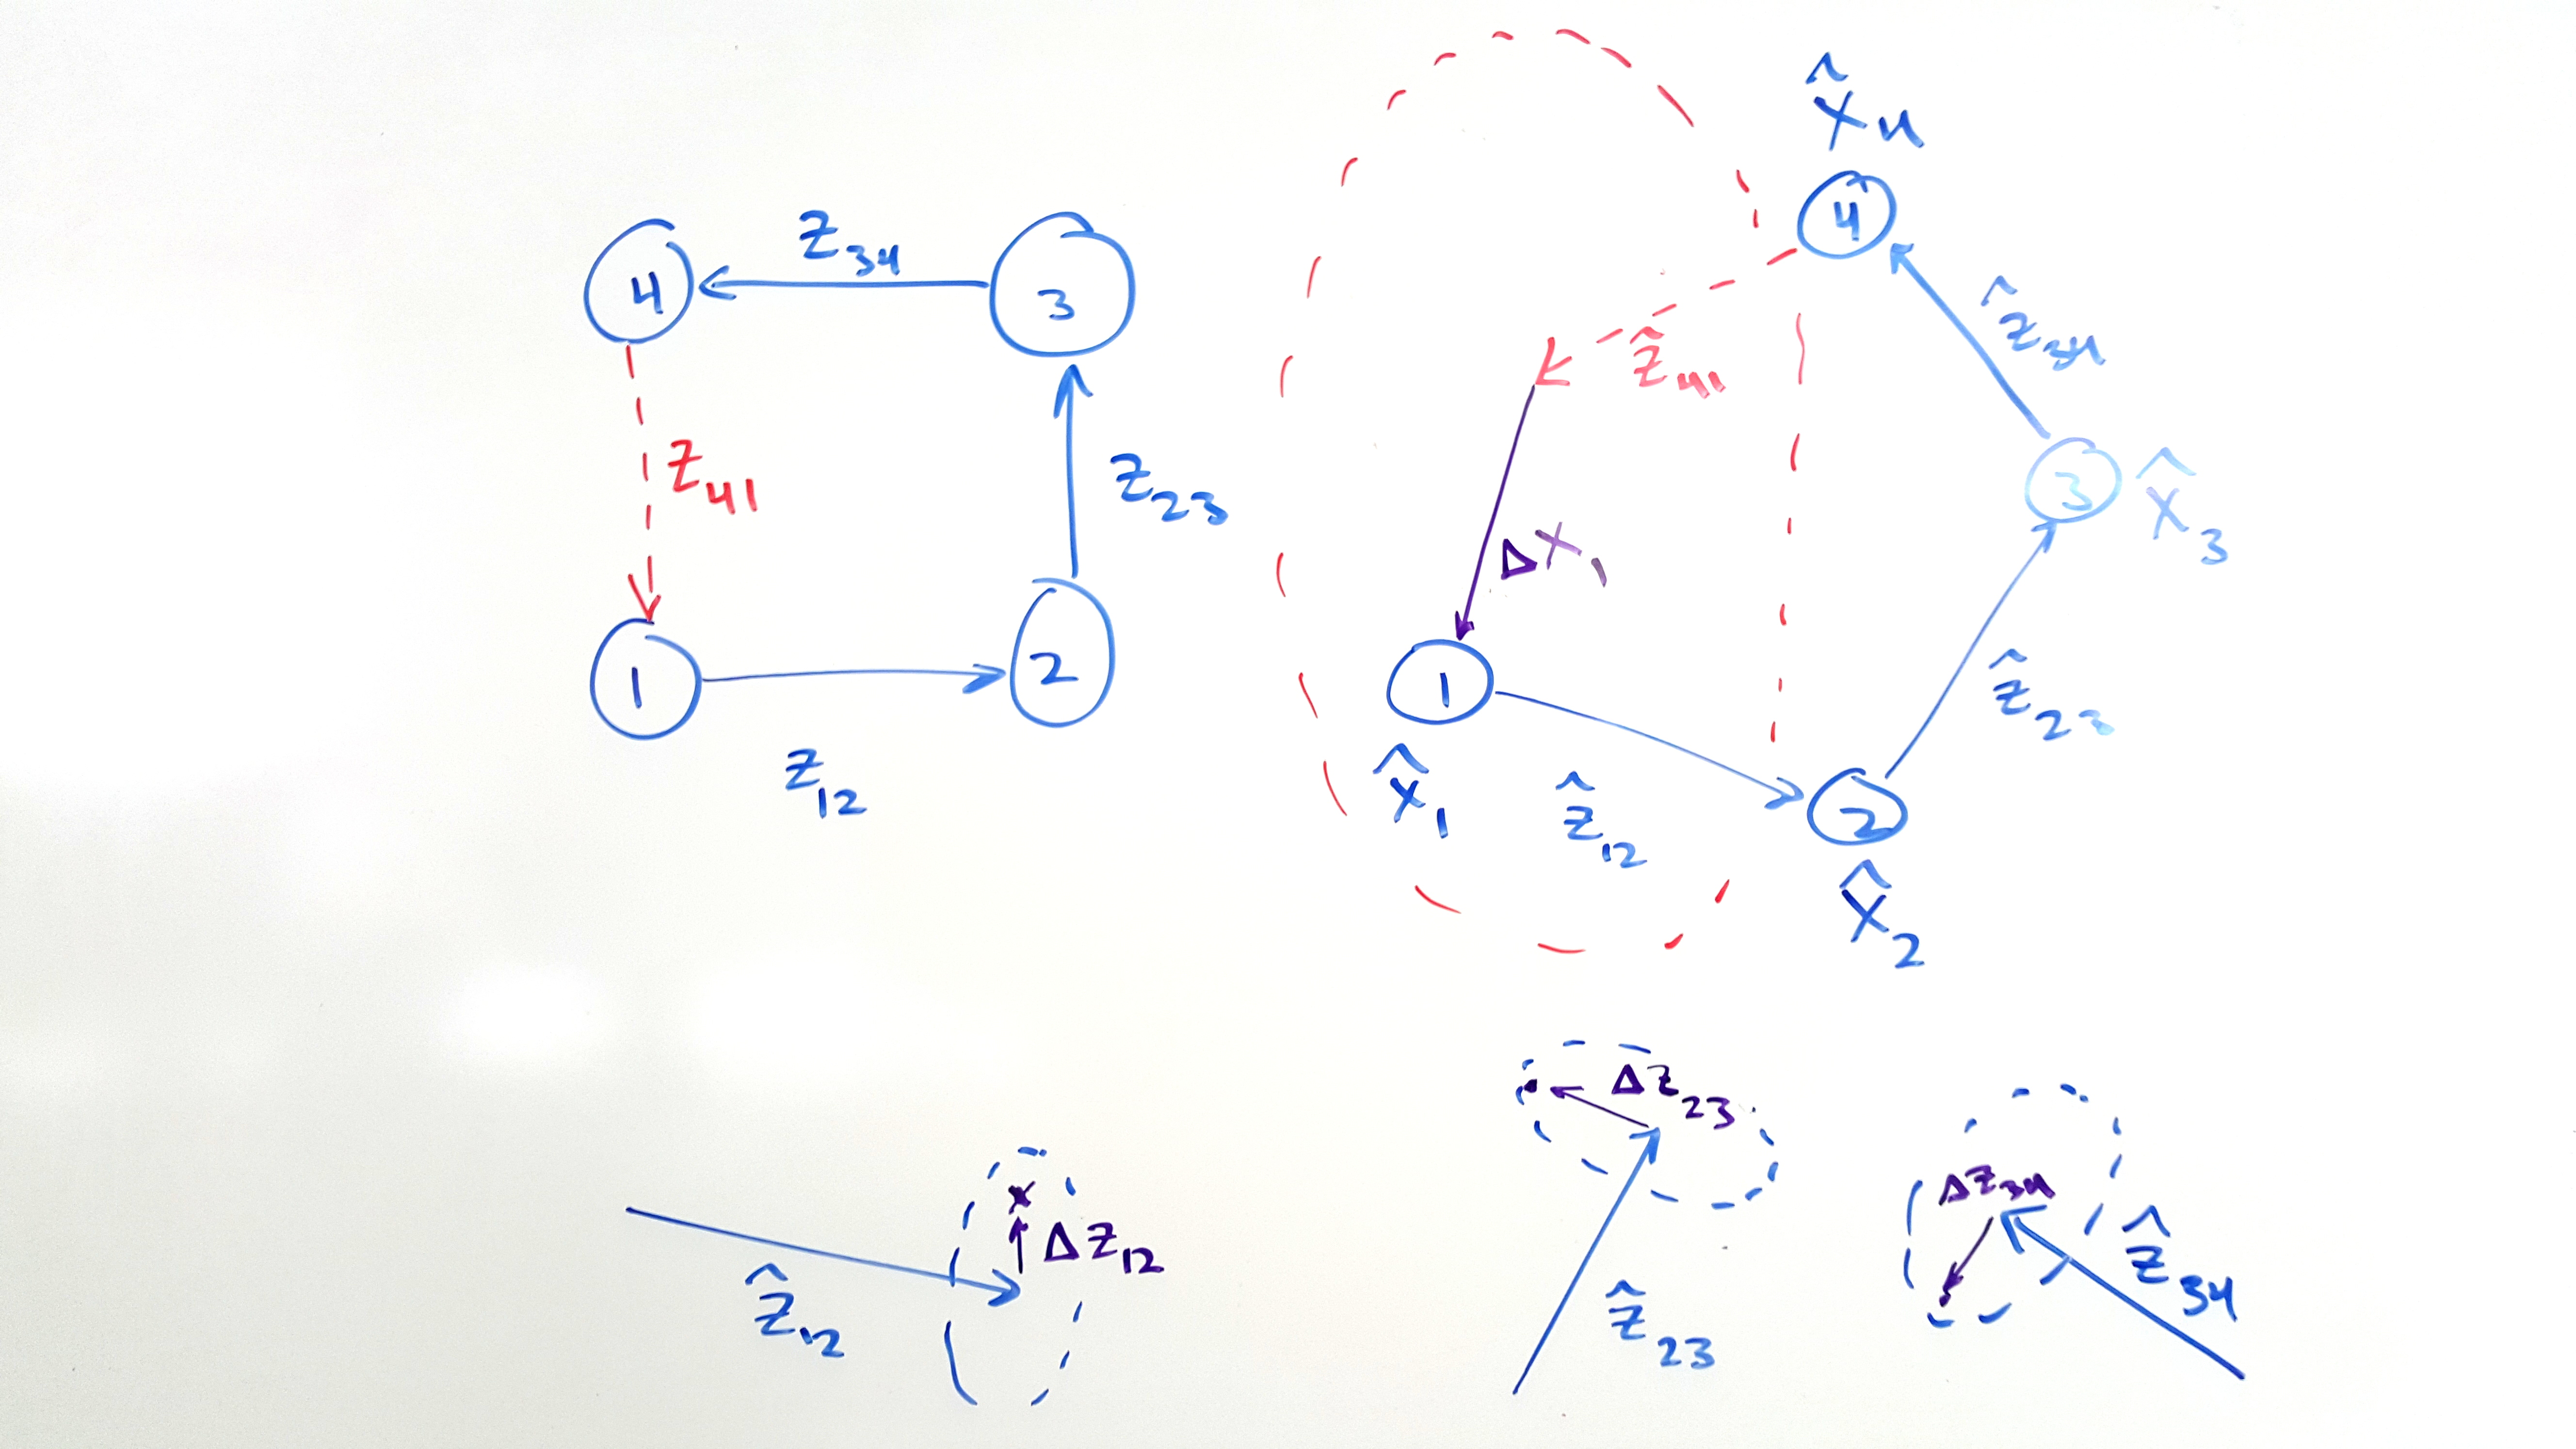
\includegraphics[width=0.7\textwidth]{figures/linearization.jpg}
  \caption{Optimizing over relative edge constraints as oppposed to global pose prevents optimization over uncertainty which has been compounded over a chain of odometry edges.  This reduces the magnitude of corrections to edge measurements and also reduces linearization errors.  Note the size of $\Delta\textbf{x}_1$ in the global update vs the incremental edge updates $\Delta \e_{ij}$.  Also note the size of the uncertainty about $\textbf{x}_1$ vs the uncertainty estimate about each edge $\e_{ij}$.  Because the uncertainty estimates are by nature much smaller for edges, linearization errors are typically smaller.}
  \label{fig:linearization}
\end{figure}

We wish to find the optimal update $\Delta\e^*$ to our initial edge estimate. Letting $\eest^+ = \eest + \Delta\e$ and $\eest_{a-z}^+ = h(\eest_{a-z},\Delta\e)$ we see
\begin{align*}
  F(\eest^+,\emeas) &= \sum_{\{i,j\} \in \mathcal{O}} (\eest_{ij} + \Delta\e_{ij}-\emeas_{ij})^\top\Omega_{ij}(\eest_{ij} + \Delta\e_{ij}-\emeas_{ij}) + \sum_{\{a,z\} \in \mathcal{L}} (\eest_{a-z}^+-\emeas_{az})^\top\Omega_{az}(\eest_{a-z}^+-\emeas_{az}) \\
  &= (\eest+\Delta\e-\emeas)^\top\boldsymbol{\Omega}(\eest+\Delta\e-\emeas) + \sum_{\{a,z\} \in \mathcal{L}} (h(\eest_{a-z},\Delta\e)-\emeas_{az})^\top\Omega_{az}(h(\eest_{a-z},\Delta\e)-\emeas_{az})
\end{align*}

where

\begin{align*}
  \boldsymbol{\Omega} &= \left[\begin{array}{ccc}
  \Omega_{01} & \mathbf{0} & \mathbf{0} \\
  \mathbf{0}  & \ddots     & \mathbf{0} \\
  \mathbf{0}  & \mathbf{0} & \Omega_{e-1,e}\\
  \end{array}\right].
\end{align*}

Taking the derivative of the cost function with respect to $\Delta\e$ and setting it equal to zero will allow us to solve for the optimal edge update $\Delta\e^*$.
\begin{align*}
  \dfrac{\partial F(\eest^+,\emeas)}{\partial \Delta\e} = \mathbf{0}^\top \\
  2 (\eest+\Delta\e^*-\emeas)^\top \boldsymbol{\Omega} \frac{\partial (\eest+\Delta\e-\emeas)}{\partial \Delta\e}
    + \sum_{\{a,z\} \in \mathcal{L}} 2
  (h(\eest_{a-z},\Delta\e^*)-\emeas_{az})^\top \Omega_{az}
  \frac{\partial h(\eest_{a-z},\Delta\e)}{\partial \Delta\e}
  = \mathbf{0}^\top
  \\
  (\eest+\Delta\e^*-\emeas)^\top \boldsymbol{\Omega}
  + \sum_{\{a,z\} \in \mathcal{L}}
  (h(\eest_{a-z},\Delta\e^*)-\emeas_{az})^\top \Omega_{az}
  \frac{\partial h(\eest_{a-z},\Delta\e)}{\partial \Delta\e}
  = \mathbf{0}^\top.
\end{align*}

Transposing both sides, noting that the information matrices are symmetric results in the following expression for the edge update:
\begin{align}
  \boldsymbol{\Omega} (\eest+\Delta\e^*-\emeas)
  + \sum_{\{a,z\} \in \mathcal{L}}
  \frac{\partial h(\eest_{a-z},\Delta\e)}{\partial \Delta\e}^\top \Omega_{az} (h(\eest_{a-z},\Delta\e^*)-\emeas_{az})
  = \mathbf{0}.
  \label{eq:edge_update}
\end{align}

The first term in Eq~\ref{eq:edge_update} causes the optimization to respect the odometry constraints; it is always linear with respect to $\Delta\e$ even when the underlying edges are nonlinearly coupled. The second term is a function of the set of edges found in the various loop closures $\mathcal{O_L}$. As a result, any edge not found in a loop closure can be trivially solved for directly using the first term. We see
\begin{align*}
  \Delta\e_{ij}^* = \emeas_{ij} -\eest_{ij}
  \end{align*}
  such that
  \begin{align*}
  \eest_{ij}^+ = \emeas_{ij}  \text{ for } \{i,j\} \notin \mathcal{O_L}.
\end{align*}
In other words, any edge estimate that is not part of a redundant path is driven to its original measured state, and in no other way influence the optimization. We can finally move all constant terms to the right-hand side of the equation and write the final cost function.
\begin{align}
  \boldsymbol{\Omega} \Delta\e^*  + \sum_{\{a,z\} \in \mathcal{L}}
  \frac{\partial h(\eest_{a-z},\Delta\e)}{\partial \Delta\e}^\top
  \Omega_{az}(h(\eest_{a-z},\Delta\e^*)-\emeas_{az})
  &= -\boldsymbol{\Omega}(\eest -\emeas)
  \label{eqn:opt}
\end{align}

To solve Eq.~\ref{eqn:opt}, we will linearize the system about current estimate for all edge constraints and perform Gauss-Newton optimization.  Let us define

\begin{align*}
  \mathbf{H}_{az} = \frac{\partial h(\eest_{a-z},\Delta\e)}{\partial \Delta\e} \mid_{\Delta\e = \mathbf{0}}
\end{align*}

such that the second-order approximation of the compounding of a series of edges in a non-trivial space, like $SE(2)$, can be shown as follows:

\begin{align*}
  h(\eest_{a-z},\Delta\e) &= (\eest_{ab} + \Delta\e_{ab}) \circ (\eest_{bc} + \Delta\e_{bc}) \circ ... \circ (\eest_{yz} + \Delta\e_{yz})\\
   &\approx
  h(\eest_{a-z},\mathbf{0}) + \mathbf{H}_{az} \Delta\e,
\end{align*}

and we will use the first order approximation for the partial
\begin{align*}
  \frac{\partial h(\e_{a-z},\Delta\e)}{\partial \Delta\e} &\approx \mathbf{H}_{az}.
\end{align*}

With this approximation, Equation \ref{eqn:opt} simplifies to

\begin{align}
  \left(\boldsymbol{\Omega} + \sum_{\{a,z\} \in \mathcal{L}}
  \mathbf{H}_{az}^\top
  \Omega_{az}\mathbf{H}_{az} \right) \Delta\e^*
  &= -\boldsymbol{\Omega}(\eest -\emeas) - \sum_{\{a,z\} \in \mathcal{L}}
  \mathbf{H}_{az}^\top
  \Omega_{az}(h(\eest_{a-z},\mathbf{0}) -\emeas_{az})
  \label{eqn:3d_opt}
\end{align}

\subsection{Relative Edge Optimization in $SE(2)$}
\label{sec:relative_edge_optimization_in_se2}

Take the example of a 3 DoF robot which follows the standard unicycle model, where edges are defined as $\e_i = \left[\begin{array}{ccc} f_i & r_i & \theta_i \end{array}\right]^\top$ where $f$ and $r$ represent forward and right motion and $\theta$ represents a change in bearing. In this case translational motion is coupled with heading. Let us first consider the simple case of a single loop closure after a string of edges, which could be described graphically as shown in~\ref{fig:pose_graph}.  In this case, the series of edges can be represented as a series of transformation matrices as follows:

\begin{align*}
	h(\eest_{a-z},\Delta\e) =  \left[\begin{array}{c}
	T_{az,13} \\ T_{az,23} \\ \sum_{i \in \{a,z\}} \left( \theta_i + \Delta\theta_i \right)
	\end{array}\right]
\end{align*}

where $T_{ij}$ is the  homogeneous transform matrix with the form

\begin{align*}
  T_{ij} &= \left[\begin{array}{ccc}
  \cos(\theta_i + \Delta\theta_i) & -\sin(\theta_i + \Delta\theta_i) & f_i + \Delta f_i \\
  \sin(\theta_i + \Delta\theta_i) &  \cos(\theta_i + \Delta\theta_i) & r_i + \Delta r_i \\ 0 & 0 & 1
\end{array}\right] \in \mathbb{R}^{3 \times 3}
\end{align*}

and compounds according to

\begin{align*}
  T_{az} &= T_{ab} T_{bc} T_{cd} ... T_{yz}.
\end{align*}

Note that bearing angle just sums between edge compounding through multiplication of the rotation part of the transform.

\begin{figure}
  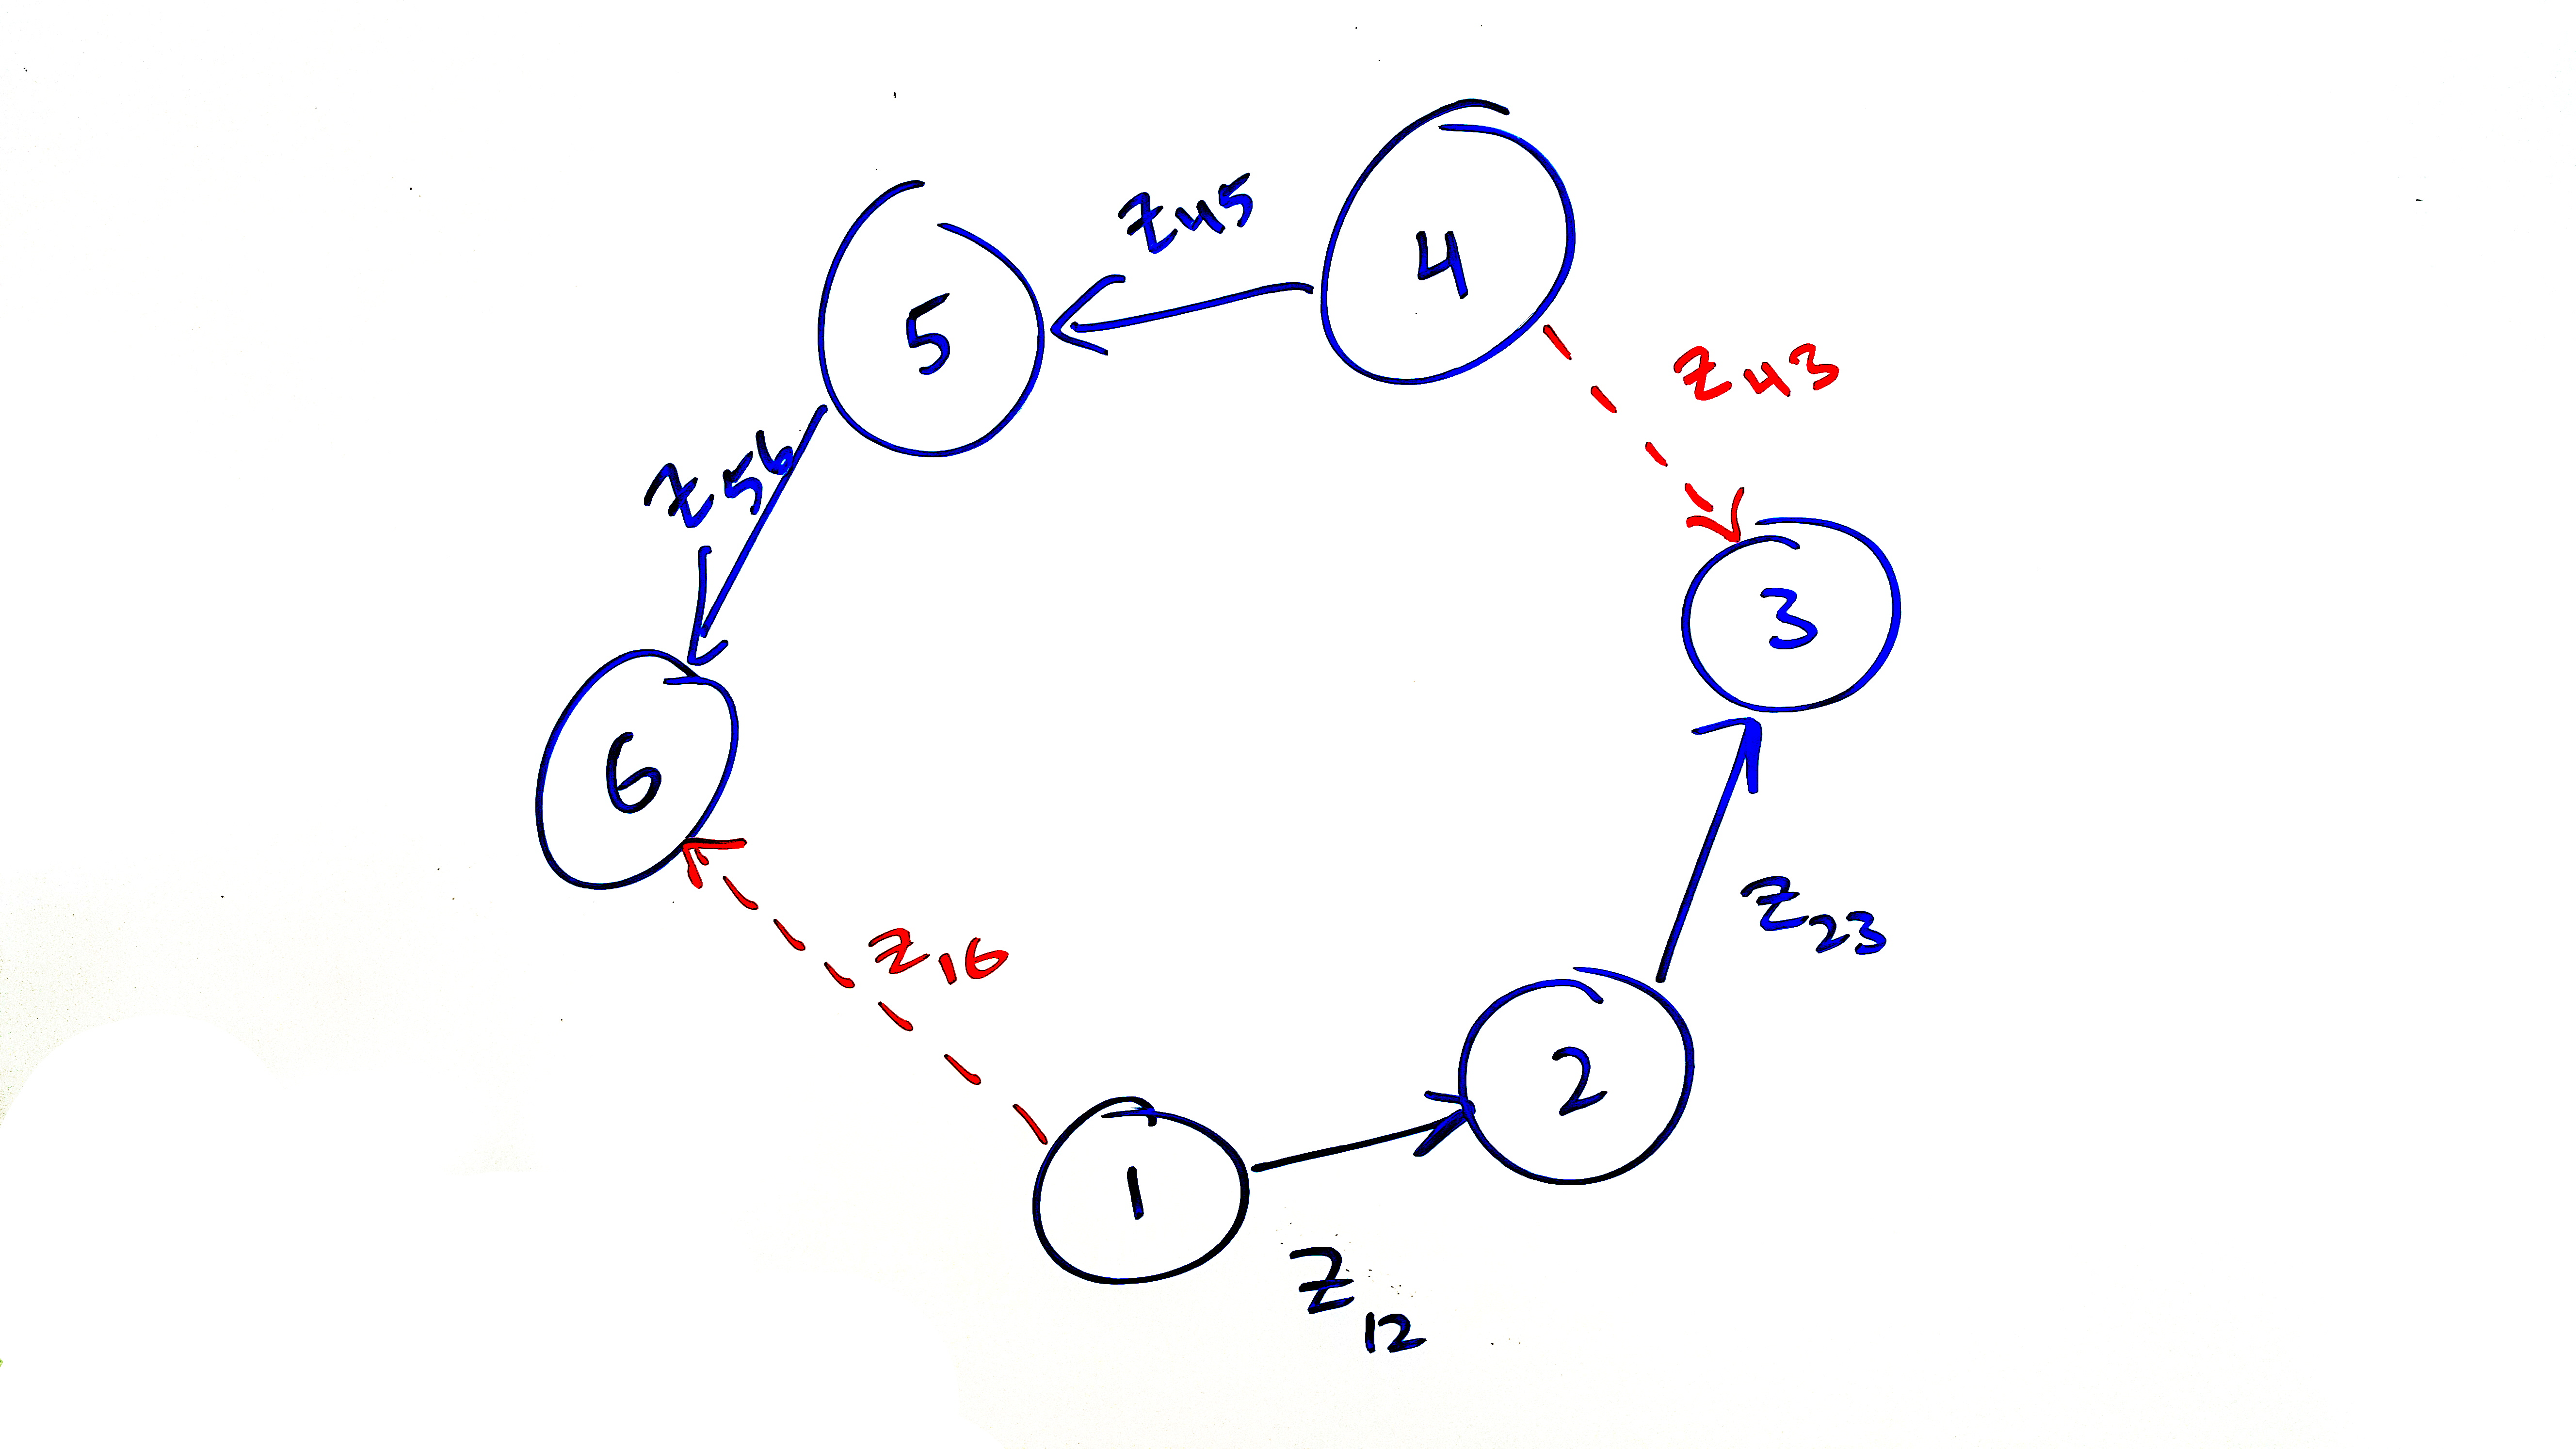
\includegraphics[width=0.7\textwidth]{figures/multiple_lc.jpg}
  \caption{A loop closure with multiple loop closures and reversed edges}
  \label{fig:reversed_pose_graph}
\end{figure}

The Jacobian $\mathbf{H}_{az}$ can be calculated for an arbitrary set of edges for a graph without reversed edges, like the one shown in Figure~\ref{fig:pose_graph} with algorithm~\ref{algo:non_reversed}.  More complicated loops, with multiple loop closures, such as pictured in Figure~\ref{fig:reversed_pose_graph}, may have one or more of the edges reversed.  In this case, the edge string must be compounded after first inverting the reversed edges.  This also causes further complications in the calculation of the Jacobian $\mathbf{H}_{az}$.  Algorithm~\ref{algo:reversed} can be used to calculate $\mathbf{H}_{az}$ in this case.

\begin{algorithm}[H]
  \caption{Jacobian Calculation for a cycle without reversed edges}\label{algo:non_reversed}
  \begin{algorithmic}[1]
    \State $\dfrac{\partial \Delta t_{a-z}}{\partial \Delta t_{1,2}} = I$
    \For{$\e_{ij} \in \mathcal{L}$}
      \State $\dfrac{\partial \Delta t_{a-z}}{\partial \Delta t_{ij}} = \prod_{\{m,n\} < \{i,j\}} R_{m,n}$
    \EndFor
    \For{$\e_{ij} \in \mathcal{L}$}
      \State $\dfrac{\partial \Delta t_{a-z}}{\partial \theta_{ij}} = \sum_{\{m,n\} >= \{i,j\}} \dfrac{\partial \Delta t_{a-z}}{\partial \Delta t_{mn}} \Delta t_{mn}$
      \State $\dfrac{\partial \theta_{a-z}}{\partial \theta_{ij}} = 1$
      \State $\dfrac{\partial \Delta t_{a-z}}{\partial \theta_{ij}} = \textbf{0}$
    \EndFor
  \end{algorithmic}
\end{algorithm}

\begin{algorithm}[H]
  \caption{Jacobian Calculation for a pose graph cycle with reversed edges}\label{algo:reversed}
  \begin{algorithmic}[1]
    \If{ dir$\left( \e_{10} \right) < 0$ }
      \State $\dfrac{\partial \Delta t_{a-z}}{\partial \Delta t_{1,2}} = -R_{12}$
    \Else
      \State $\dfrac{\partial \Delta t_{a-z}}{\partial \Delta t_{1,2}} = I$
    \EndIf
    \For{$\e_{ij} \in \mathcal{L}$}
      \If{ dir$\left( \e_{ij} \right) > 0$ }
        \State $\dfrac{\partial \Delta t_{a-z}}{\partial \Delta t_{ij}} = \prod_{\{m,n\} < \{i,j\}} R_{m,n}$
      \Else
        \State $\dfrac{\partial \Delta t_{a-z}}{\partial \Delta t_{ij}} = -\prod_{\{m,n\} \leq \{i,j\}} R_{m,n}$
      \EndIf
    \EndFor
    \For{$\e_{ij} \in \mathcal{L}$}
      \If{ dir$\left( \e_{ij} \right) > 0$ }
        \State $\dfrac{\partial \Delta t_{a-z}}{\partial \theta_{ij}} = \sum_{\{m,n\} > \{i,j\}} \dfrac{\partial \Delta t_{a-z}}{\partial \Delta t_{mn}} \Delta t_{mn}$
      \Else
        \State $\dfrac{\partial \Delta t_{a-z}}{\partial \theta_{ij}} =
        - \sum_{\{m,n\} \geq \{i,j\}} \dfrac{\partial \Delta t_{a-z}}{\partial \Delta t_{mn}} \Delta t_{mn}$
      \EndIf
      \State $\dfrac{\partial \theta_{a-z}}{\partial \theta_{ij}} = $dir$\left( \e_{ij} \right)$
      \State $\dfrac{\partial \Delta t_{a-z}}{\partial \theta_{ij}} = \textbf{0}$
    \EndFor
  \end{algorithmic}
\end{algorithm}
